\section{Theorie}
\label{sec:theorie}

    Im folgenden Abschnitt sollen die theoretischen Grundlagen der Entstehung von Röntgenstrahlung,
    die Gestalt des Röntgen- und Absorptionsspektrums,
    sowie die Bragg-Reflexion erläutert werden.

\subsection{Das Röntgenspektrum}

    Röntgenstrahlung entsteht in einer Röntgenröhre.\\

    \begin{figure}
        \centering
        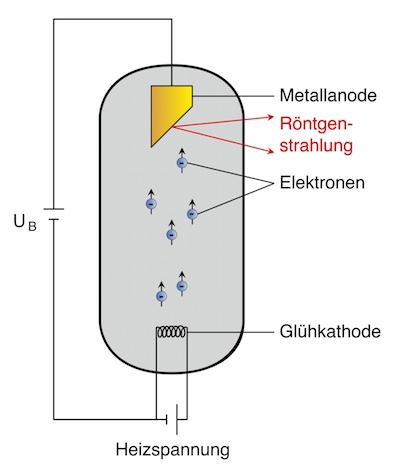
\includegraphics[width=0.5\textwidth]{content/img/Roentgenroehre.jpg}
        \caption{Der Aufbau einer Röntgenröhre. \cite{roentgenroehre}}
        \label{fig:Röntgenröhre}
    \end{figure}

    In einer evakuierten Röhre werden mithilfe des glühelektrischen Effekts an einer negativ geladenen Kathode Elektronen ausgelöst.
    Die Elektronen werden in einem elektrischen Feld zu einer positiv geladenen Anode hin beschleunigt,
    wobei ihre potentielle (elektrische) Energie in kinetische Energie umgewandelt wird.
    Wenn die Elektronen auf die Anode auftreffen,
    werden sie so stark abgebremst,
    dass sie Energie in Form von Strahlung abgeben.
    Es wird dabei zwischen kontinuierlicher Bremsstrahlung und charakteristischer Röntgenstrahlung unterschieden.

    \phantomsection
    \label{sec:theorie:bremsspektrum}
    Das \textbf{kontinuierliche Bremsspektrum} entsteht durch die aus Coulombkräften resultierende Abbremsung.
    Die Elektronen geben Energie in Form eines Photons,
    auch Röntgenquant genannt,
    ab.
    Dabei muss das Elektron jedoch nicht seine gesamte Energie abgeben,
    sondern kann einen Teil als kinetische Energie behalten,
    was zu einem kontinuierlichen Spektrum führt,
    da jedes Elektron einen unterschiedlichen Energiebetrag abgeben kann,
    wie in \autoref{fig:Bremsspektrum} gezeigt.

    \begin{figure}
        \centering
        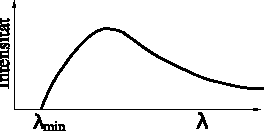
\includegraphics[width=0.4\textwidth]{content/img/Abb_1.pdf}
        \caption{Das kontinierliche Spektrum der Bremsstrahlung. \cite{versuchsanleitung}}
        \label{fig:Bremsspektrum}
    \end{figure}

    Die minimale Wellenlänge $\lambda_\text{min}$ beschreibt den Fall,
    bei dem das Elektron seine gesamte kinetische Energie abgibt und diese in Strahlungsenergie umgewandelt wird.
    Es gilt
    \begin{equation*}
        \lambda_\text{min} = \frac{hc}{eU_\text{B}} \; ,
    \end{equation*}
    mit der Elementarladung $e$ des Elektrons und der Beschleunigungsspannung $U_\text{B}$.
    %Die Wellenlänge beschreibt die größte Energie,
    %die ein Teilchen als Quant übertragen kann.
    %%Das habe ich damals im LK so gelernt, ich weiß nicht ob wir das reinnehmen sollen, es steht so nicht in der Anleitung.

    \phantomsection
    \label{sec:theorie:char_spektrum}
    Das \textbf{charakteristische Spektrum} kommt durch Ionisierung der Anodenatome zustande,
    wenn die Elektronen auf die Anode treffen.
    Dabei entsteht eine Lücke auf einer der inneren Schalen,
    sodass ein Elektron von einem höheren Energieniveau in die Lücke zurückfallen kann.
    Die dabei freiwerdende Energie wird in Form eines Röntgenquants ausgesendet,
    welches genau die Energie aus der Energiedifferenz
    \begin{equation*}
        E = h \nu = E_\text{m} - E_\text{n}
    \end{equation*}
    besitzt.
    Die freiwerdende Energie ist abhängig vom Anodenmaterial,
    was zu einem diskreten Energiespektrum führt.
    Die entstehenden scharfen Linien des Spekrums werden mit
    $K_{\symup{\alpha}}$, $K_{\symup{\beta}}$, $L_{\symup{\alpha}}$ bezeichnet,
    abhängig von der Schale $K$, $L$, $M$,
    auf die das Elektron zurückfällt.
    Der Index $\alpha$, $\beta$ bezeichnet die Ursprungs-Schale des Elektrons.
    Die Elektronen in den inneren Schalen werden von denen aus den äußeren Schalen abgeschirmt,
    sodass sich die Bindungsenergie der einzelnen Elektronen auf den Schalen unterscheidet.
    Für die $n$-te Schale ergibt sich eine Energie von
    \begin{equation}
        \label{eqn:E_n}
        E_\text{n} = - R_\infty z_{\text{eff}}^2 \cdot \frac{1}{n^2} \ ,
    \end{equation}
    mit der Rydbergenergie $R_\infty = \SI{13.6}{\electronvolt}$,
    der effektiven Kernladungszahl $z_{\text{eff}} = z - \sigma$ und der Abschirmkonstante $\sigma$.
    Die Spektrumslinien der äußeren Elektronen teilen sich in mehrere eng aneineranderliegende Linien auf,
    da die Bindungsenergien dieser Elektronen sich durch Bahndrehimpuls und Elektronenspin unterscheiden.
    Diese Reihe von beieinanderliegenden Linien wird als Feinstruktur bezeichnet.
    Die genaue Energie der einzelnen Linien kann mithilfe der Sommerfeld'schen Feinstrukturformel berechnet werden:
    \begin{equation}
        \label{eqn:Feinstrukturformel}
        E_\text{n,j} = - R_\infty
        \left(z_{\text{eff},1}^2 \cdot \frac{1}{n^2} + \alpha^2 \cdot \frac{1}{n^3}
          \left( \frac{1}{j+\frac{1}{2}}- \frac{3}{4n} \right)
        \right) \; .
    \end{equation}
    Hierbei stellt $\alpha = \frac{1}{137}$ die Sommerfeld'sche Feinstrukturkonstante und $j$ den Gesamtdrehimpuls des Elektrons dar.
    Für die $K$-Schale kann die Energie unter Vernachlässigung des Drehimpulses mithilfe von
    \begin{align}
        % Wer schön sein will, muss leiden… ;)
        \nonumber
        E_\text{K,abs} &= R_\infty (z - \sigma_1)^2
        \\
        \label{eqn:EnergieKalpha}
        E_{\mathmakebox[0pt][l]{\text{K},\symup{\alpha}}\phantom{\text{K,abs}}} &= R_\infty \Bigl(\frac{1}{n}\Bigr)^2 \cdot (z - \sigma_1)^2 -R_\infty \Bigl(\frac{1}{m}\Bigr)^2 \cdot (z - \sigma_2)^2
        \\
        \label{eqn:EnergieKbeta}
        E_{\mathmakebox[0pt][l]{\text{K},\symup{\beta}}\phantom{\text{K,abs}}} &= R_\infty \Bigl(\frac{1}{n}\Bigr)^2 \cdot (z - \sigma_1)^2 - R_\infty \Bigl(\frac{1}{l}\Bigr)^2 \cdot (z - \sigma_3)^2
    \end{align}
    berechnet werden.\\


\subsection{Absorption von Röntgenstrahlung}

    Bei Röntgenstrahlung mit einer Energie unter $\SI{1}{\mega\electronvolt}$ sind die dominanten Prozesse der Photoeffekt und der Compton-Effekt.
    Wenn die Röntgenstrahlung auf einen Absorber trifft,
    nimmt der Absorptionskoeffizient bei zunehmender Energie ab,
    steigt aber stark an,
    sobald die Photonenenergie größer als die Bindungsenergie der ersten Schale ist,
    was in \autoref{fig:Absorption} darstellt ist.\\
    Nach dem Moseley'schen Gesetz ist die Absorptionsenergie $E_\text{K}$ proportional zum Quadrat der Ordnungszahl $Z$ des Absorbermaterials.
    Es gilt
    \begin{equation}
        E_\text{K} = R h (z - \sigma)^2
        \label{eqn:Moseley}
    \end{equation}

    \begin{figure}
        \centering
        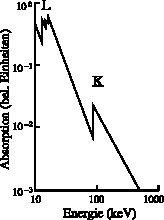
\includegraphics[width=0.3\textwidth]{content/img/Abb_2.pdf}
        \caption{Verlauf der Absorption bei steigender Energie der Röntgenstrahlung. \cite{versuchsanleitung}}
        \label{fig:Absorption}
    \end{figure}

    Die Energie der Schale,
    aus der das Elektron stammt,
    wird als $K$, $L$, $M$-Absorptionskante bezeichnet.
    Für die einzelne $K$-Kante der $K$-Schale,
    welche die Hauptquantenzahl $n=1$ besitzt,
    ergibt sich mithilfe der \autoref{eqn:Feinstrukturformel} die Abschirmkonstante
    \begin{equation}
        \label{eqn:SigmaK}
        \sigma_\text{K} = Z - \sqrt{\frac{E_\text{K}}{R_\infty} - \frac{\alpha^2 Z^2}{4}} \; ,
    \end{equation}
    mit der Ordnungszahl $Z$ des zu untersuchenden Materials.

    % So kann man auch seine Zeit verbringen: „Voodoo programming“
    \newcommand{\romansub}[1]{\mathrm{\uppercase\expandafter{\romannumeral #1}}}

    Die $L$-Schale besitzt drei Kanten,
    $L_{\romansub{1}}$, $L_{\romansub{2}}$ und $L_{\romansub{3}}$,
    wobei in diesem Versuch nicht zwischen $L_{\romansub{1}}$ und $L_{\romansub{2}}$ unterschieden werden kann,
    sodass sich mit $\symup{\Delta} E_\text{L} = E_{\text{L}_{\romansub{2}}} - E_{\text{L}_{\romansub{3}}}$
    für die Abschirmkonstante
    \begin{equation}
        \sigma_\text{L} = Z - \sqrt{\frac{4}{\alpha}
        \sqrt{\frac{\symup{\Delta}E_\text{L}}{R_\infty}} - \frac{5\symup{\Delta}E_\text{L}}{R_\infty}}
        \sqrt{1 + \frac{19}{32}\alpha^2 \frac{\symup{\Delta}E_\text{L}}{R_\infty}}
    \end{equation}
    ergibt.


\subsection{Untersuchung der Röntgenstrahlung mithilfe der Bragg'schen Reflexion}

    Die Wellenlängen und damit auch die Energien der Röntgenstrahlung können mithilfe von Reflexion untersucht werden.
    Die Röntgenstrahlung wird aus der Röntgenröhre (siehe \autoref{fig:Röntgenröhre}) auf einen Gitterkristall (hier ein LiF-Kristall) gelenkt.
    An den Atomen des Kristalls,
    welche einen Abstand $d$ voneinander haben,
    werden die Strahlen reflektiert.
    \begin{figure}
        \centering
        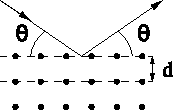
\includegraphics[width=0.3\textwidth]{content/img/Abb_3.pdf}
        \caption{Reflexion der Röntgenstrahlung am Gitterkristall. \cite{versuchsanleitung}}
        \label{fig:BraggReflexion}
    \end{figure}

    Bei einem sogenannten Glanzwinkel $\theta$ kommt es zu konstruktiver Interferenz.
    Die Beziehung zwischen Glanzwinkeln der Beugungsordnung $n$ und der Wellenlänge $\lambda$
    ist durch die Bragg-Bedingung
    \begin{equation}
        \label{eqn:BraggBedingung}
        2 d \sin{\theta} = n \cdot \lambda
    \end{equation}
    gegeben.
